\documentclass{article}
\usepackage{graphicx}  
\usepackage{caption}   
\usepackage{hyperref}  

\title{Analysis of Heart Disease Dataset}
\author{Aviral Saxena}
\date{\today}

\begin{document}
	
	\maketitle
	
	\section{Introduction}
	
	In this document, we analyze various aspects of a heart disease dataset. Below, we provide visualizations that help in understanding the relationship between various factors, including age and cholesterol levels in individuals without heart disease.
	
	\section{Correlation between Age and Cholesterol}
	
	Figure~\ref{fig:age_vs_chol} shows the correlation between age and cholesterol levels for individuals who do not have heart disease. We observe a general trend that provides insights into how these two variables are related in the absence of heart disease.
	
	\begin{figure}[h!]
		\centering
		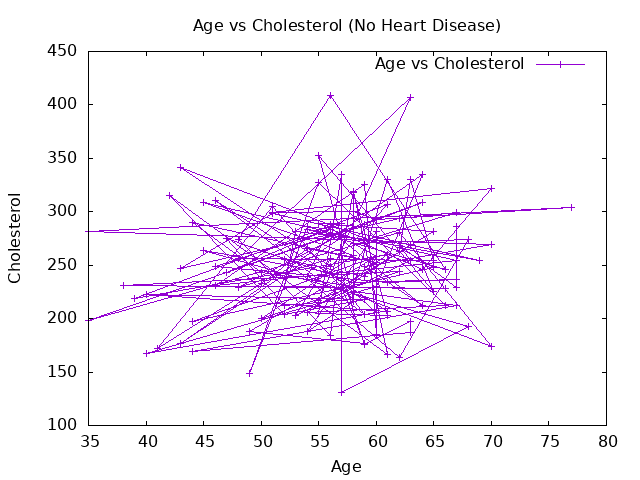
\includegraphics[width=0.7\textwidth]{ques4c.png}
		\caption{Age vs Cholesterol for individuals without heart disease}
		\label{fig:age_vs_chol}
	\end{figure}
	
	\section{Other Visualizations}
	
	We also include other visualizations to show different relationships in the dataset.Like shown in fig \ref{fig:image2} fig \ref{fig:image3} and fig\ref{fig:image4}
	
	\begin{figure}[h!]
		\centering
		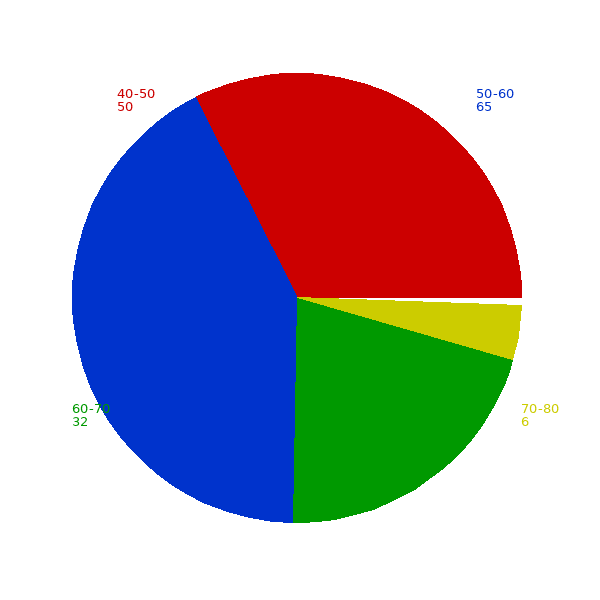
\includegraphics[width=0.7\textwidth]{ques4d.png}
		\caption{Visualization of another dataset correlation}
		\label{fig:image2}
	\end{figure}
	
	\begin{figure}[h!]
		\centering
		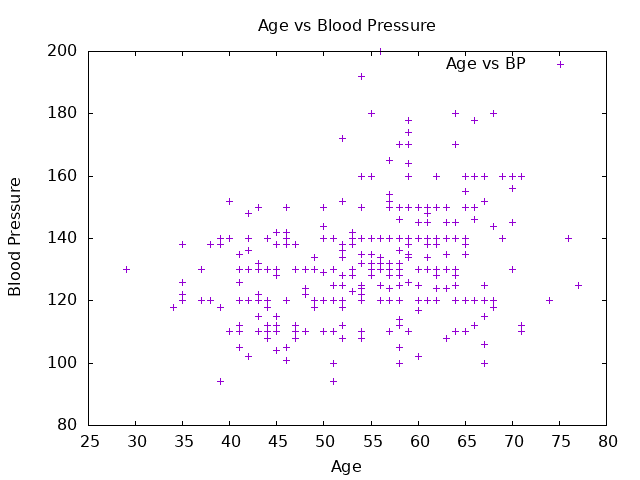
\includegraphics[width=0.7\textwidth]{ques4b.png}
		\caption{Scatter plot for variable comparison}
		\label{fig:image3}
	\end{figure}
	
	\begin{figure}[h!]
		\centering
		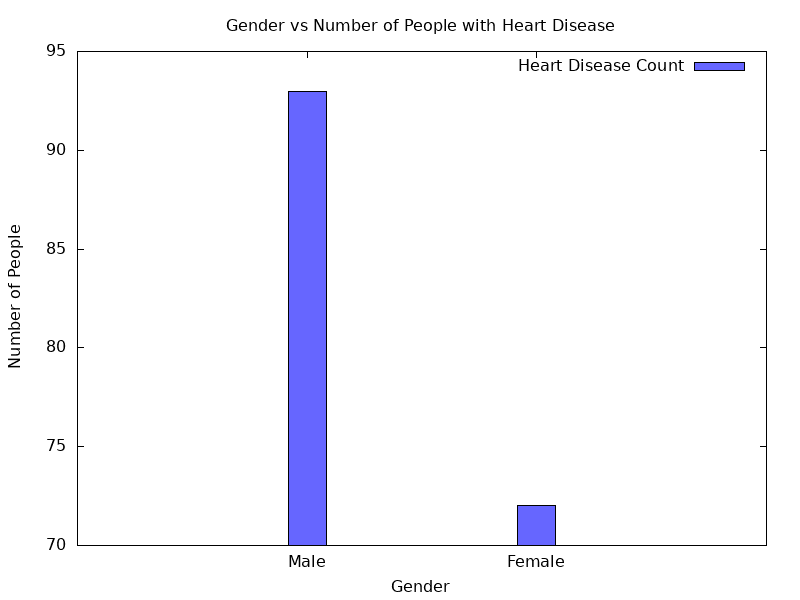
\includegraphics[width=0.7\textwidth]{ques4a.png}
		\caption{Histogram showing data distribution}
		\label{fig:image4}
	\end{figure}
	
	
	
	\section{Conclusion}
	
	These plots provide valuable insights into the relationship between age, cholesterol, and other factors that may contribute to heart disease. Further analysis can help in developing predictive models for heart disease risk.
	
\end{document}